\chapter{Results}
\label{chapter:results}
In this chapter, we perform a Bayesian analysis on the heavy-flavor transport model and extract the heavy quark transport coefficients.
I would like to present both our earlier extraction using older models and the present extract to emphasize the latest improvements.

\section{Lessons from earlier extractions of $\hat{q}_Q$}
In an earlier publication \cite{Ke:2018tsh}, we used a linearized Boltzmann model with the coherence factor approach to implement the LPM effect.
The coherence factor approach, described in section  \ref{section:compare_former} modifies the incoherent gluon radiation rate with an interference factor $2(1-\cos\Delta t/\tau_f)$. 
It also uses a multiple emission prescription by resetting $\Delta t=0$ after every emission.
We have commented on its advantages and disadvantages in \ref{section:compare_former}.

The heavy quark initial momentum distribution was obtained from the FONLL calculation.
We have already commented on the advantages and disadvantages of these choices.
Two different sets of nuclear PDF--EPPS and nCTEQ15--were used to represent the uncertainty from the cold nuclear matter effect in the $\hat{q}$ extraction.

Regarding model parameters, the one parameter for the perturbative elastic and inelastic scatterings was controlled by $1/3 < \mu < 4$ in the running coupling. 
There was an additional pure diffusion process with a diffusion constant $\kappa_{NP}$ parametized to peak at low temperature and low energy, in order to mimic the non-perturbative coupling between a low energy probe and the medium near $T_c$,
\begin{eqnarray}
\kappa_{NP} = T^3 \kappa_D \left(x_D + (1-x_D)\frac{1\textrm{ GeV}{}^2}{ET}\right).
\end{eqnarray}
The $0<\kappa_D<8$ parameter was the overall strength of the diffusion, and the $0<x_D<1$ controlled the degree of energy-temperature dependence.
One can see that in the heavy quark limit $M\rightarrow \infty$, this parametrization becomes independent of mass.
An additional parameter was the in-medium energy loss starting time $\tau_0$ that was allowed to be tuned between $0.1$ fm/$c$ to $1.0$ fm/$c$ (before the onset of hydrodynamics).
The reason is our lack of a quantitative description of the production of color charge in the initial stages.
This starting time is a simple approximation that interactions was only turned on after $\tau_0$ when the color carries was assumed to approach a Boltzmann distribution.

The design of the four dimensional parameter space  $(\tau_0, \mu, \kappa_D, x_D)$ had 80 design points.
The computation was carried on the distributed computing system Open Science Grid \cite{Pordes:2007zzb,Sfiligoi:2010zz} using about a million CPU hours.
The observables on which we calibrated are listed in tables \ref{table:ALICE-obs} and \ref{table:CMS-obs}. 
Including, $p_T$ dependent $D$-meson nuclear modification factor $R_{AA}$ and $p_T$ dependent (event-shape-engineered) azimuthal anisotropy $v_2$.
CMS measurements of the $B^{\pm}$-meson $R_{AA}$ were also included to constrain the mass dependence of the transport coefficients.

\begin{figure}
\singlespacing
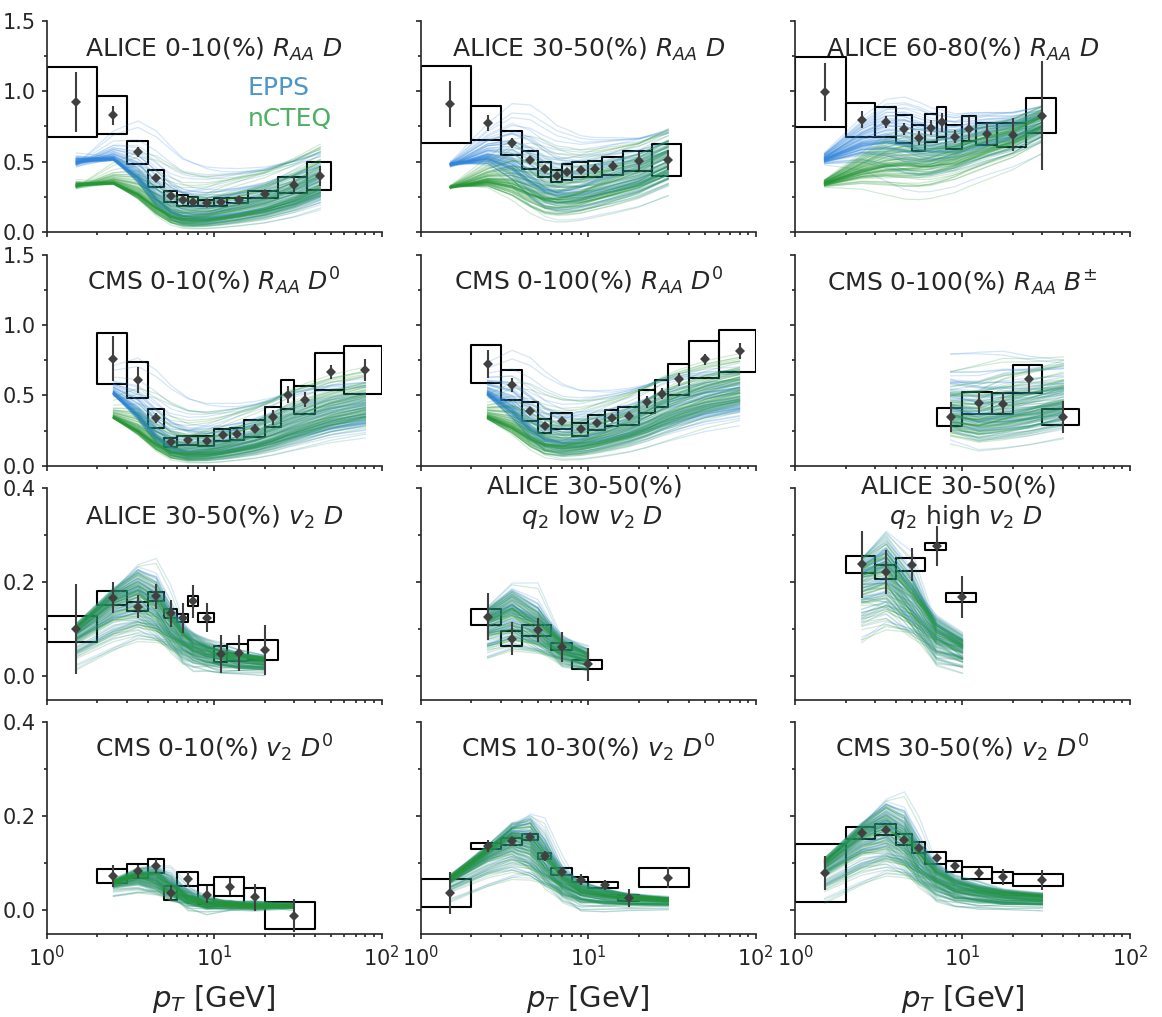
\includegraphics[width=\textwidth]{observables_design.png}
\caption[The prior distribution of calculated observables compared to data.]{The prior distribution of calculated observables compared to data. The colors labeled the use of EPPS (blue) and nCTEQ15np (green) nuclear PDF.}
\label{fig:LBT:obs_prior}
\end{figure}

\begin{figure}
\singlespacing
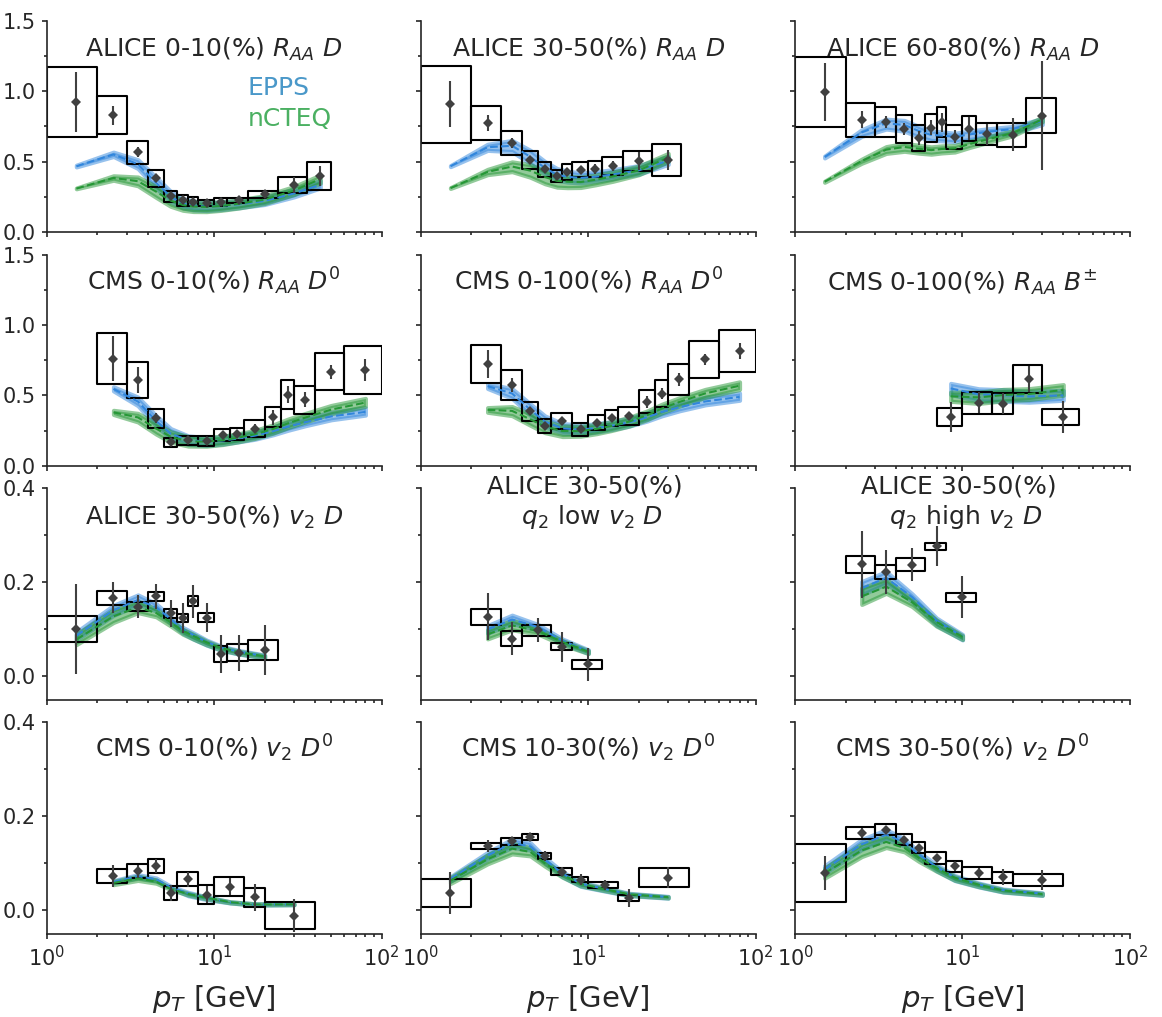
\includegraphics[width=\textwidth]{observables_posterior.png}
\caption[The 90\% credible region of the posterior distribution of observables]{The 90\% credible region of the posterior distribution of observables compared to data. The colors labeled the use of EPPS (blue) and nCTEQ15np (green) nuclear PDF.}
\label{fig:LBT:obs_posterior}
\end{figure}

The prior and the posterior of the observables before and after the calibration is shown in figures \ref{fig:LBT:obs_prior} and \ref{fig:LBT:obs_posterior}.
blue stands for using EPPS nuclear PDF and green stands for using the nCTEQnp nuclear PDF.
We found that the model after the calibration provided a good description of $R_{AA}$ and $v_2$ at the intermediate $p_T$ of the ALICE experiments.
But it did not reproduce the fast uprising shape of $R_{AA}$ at high-$p_T$ of the CMS experiment.
In addition, the model seemed to underestimate the high-$p_T$ $v_2$ of the $30-50\%$ centrality bin measured by CMS.
The model is able to explain the correlation between the D-meson $v_2$ and the event-shape, though there are still large fluctuation in the data.
The use of different nuclear PDFs had a negligible effect on $v_2$, but did affect the $R_{AA}$ at small and large $p_T$.
Another thing worth noting is that the $D$ and $B$ meson $R_{AA}$ were described at the same time.

\begin{figure}
\singlespacing
\centering
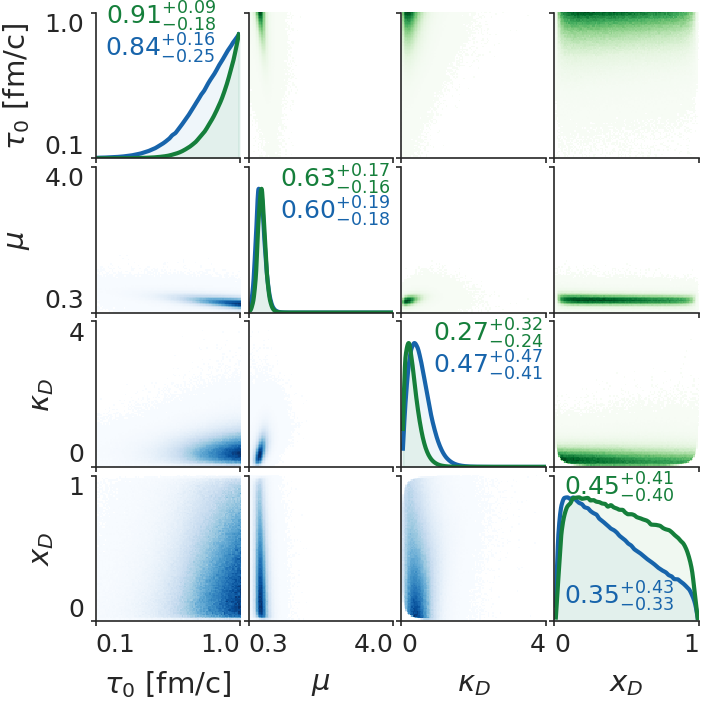
\includegraphics[width=.6\textwidth]{posterior.png}
\caption[Posteriors of single-parameter distributions (diagonal plots) and]{Posteriors of single-parameter distributions (diagonal plots) and two-parameter joint distributions (off-diagonal plots). The colors labeled the use of EPPS (blue) and nCTEQ15np (green) nuclear PDF.}
\label{fig:LBT:posterior}
\end{figure}

The inferred posterior probability distribution of the parameters is shown in the figure \ref{fig:LBT:posterior}.
The diagonal plots show single parameterized distributions, and the off-diagonal ones displays the two-parameter correlations.
We split the results that use different nuclear PDFs into the upper (EPPS, green heat map and lines) and lower (nCTEQ15np, blue heat maps and lines) triangles.
One notices that the results from different nuclear PDF are consistent within the uncertainty; therefore, from now on I shall not stress on any differences between these two sets of results, but combine them into a single distribution to fold in the PDF uncertainty.
The favored parameters are $\mu \sim 0.6$ and $\kappa_D \sim 0.4$, indicating a large in-medium $\alpha_s$ and a small amount of additional diffusion.
The typical value of $\alpha_s$ is, in fact, so large that one is let to worry about the use of weakly-coupled approaches.
For example, $\alpha_s(0.6\pi T)$ at $T=300$ MeV is 0.67, corresponding to $g \approx 3$. 
And the screening mass $m_D \sim 3.6 T$ is even larger than the average energy of the thermal partons $3T$. 
In the discussion of the next section, we will see that this problem can be somewhat alleviated, once we use the improved implementation of the LPM effect and implement a separation of soft-modes into the diffusion constant, though $g$ is still large.

\begin{figure}
\singlespacing
\centering
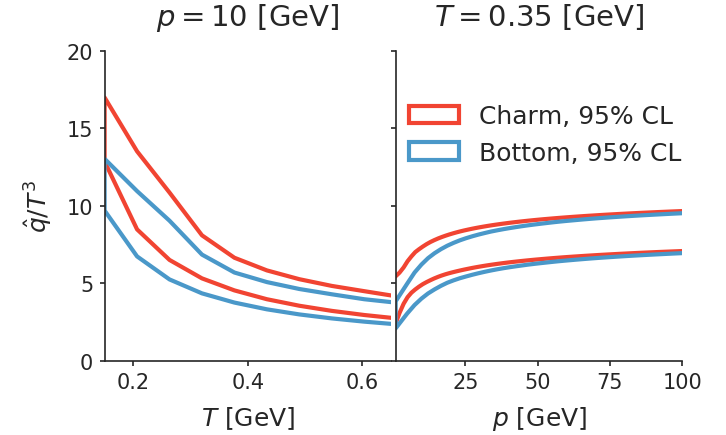
\includegraphics[width=.8\columnwidth]{qhat_p_T.png}
\caption[The 95\% credible region of the heavy quark transport coefficient]{The 95\% credible region of the heavy quark transport coefficient $\hat{q}$ extracted using the model described in \cite{Ke:2018tsh}.
The charm quark results are shown in red, and bottom results in blue.
The difference coming from using different nuclear PDF has been marginalized into the uncertainty bands.
Left plot: the temperature dependence at $p=10$ GeV. Right plot: the momentum dependence at $T=0.35$ GeV.
}\label{fig:LBT:posterior_qhat}
\end{figure}

\paragraph{Transport coefficients} In this analysis, the heavy quark transport coefficient $\hat{q}$ is computed by adding up the momentum broadening from both the scattering and the parametric diffusion,
\begin{eqnarray}\label{eq:qhat}
\hat{q} &=& 2T^3\kappa_D\left(x_D + (1-x_D)\frac{\textrm{GeV}^2}{ET}\right) + \hat{q}_{\textrm{el}}.
\end{eqnarray}
In a perturbative definition of the transport coefficients, the inelastic process does not contribute to heavy quark transport coefficient at leading order. 
In figure \ref{fig:LBT:posterior_qhat}, the 95\% credible region of $\hat{q}$ is shown as a function of temperature at a fixed energy (left), and as function of energy at a fixed temperature (right).
Results for charm (red) and bottom (blue) quarks are labeled by different colors.
The mass difference only causes a small difference in $\hat{q}$.

\begin{figure}
\singlespacing
\centering
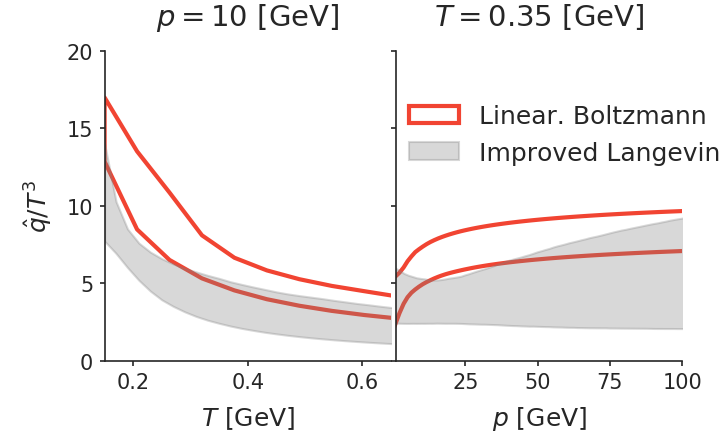
\includegraphics[width=.8\columnwidth]{qhat_compare.png}
\caption[Comparison of the 95\% credible region of the charm $\hat{q}$ using]{Comparison of the 95\% credible region of the charm $\hat{q}$ using different models. The red regions use the model described in \cite{Ke:2018tsh}, while the  shaded regions are obtained using  the improved-Langevin model \cite{Cao:2013ita}.}\label{fig:LBT:compare_qhat}
\end{figure}

\paragraph{Comparison to results from an improved-Langevin model}
The same transport coefficient is also extracted using the improved-Langevin model \cite{Cao:2013ita}.
It includes a diffusion modeling of the elastic interaction, a higher-twist single gluon emission rate, and a similar routine to implement multiple radiations.
This model is then coupled to the same medium as the one used here and compared to the same set of observables as this work does.
The resultant posterior (for charm quarks only) is shown as the shaded region in figure \ref{fig:LBT:compare_qhat}.
We see that the $\hat{q}$ extracted using the two models only overlap at the boundary of the credible region.
Their difference is comparable to the uncertainty band of either model, while both models provide a reasonable description of the data.
This suggests that the theoretical uncertainty that comes from the assumption made about the probe-medium is a significant one.
The ability to tune a switching scale parameter in the new model intends to include this type of theoretical uncertainty.

\section{Calibration using the improved transport model}
Finally, we apply the improved model to the extraction of the heavy quark transport coefficients.
Here we summarize the improvements:
\begin{itemize}
\item A more sophisticated implementation of the LPM effect to reduce modeling uncertainty of the radiative processes;
\item An interpolation between the diffusion picture and the scattering picture to take into account modeling uncertainty.
\item Separation of the high-virtuality evolution and the low-virtuality transport equation at a medium scale.
\end{itemize}

\begin{table}
\centering
\caption{Prior range of parameters}\label{table:new:prior}
\begin{tabular}{ccc}
\hline
Symbol & Description & Range \\
\hline
$\xi = \frac{\tau_0}{\tau_{\textrm{hydro}}}$ & Energy loss starting time & (.1, .9) \\
$c = \frac{Q_{\textrm{cut}}^2}{m_D^2}$ & Soft / hard switching scale & $(.1, 10.)$ \\
$R_v$ & Vacuum / Medium matching scale & $(0,7)$\\
$\mu$ & Running $\alpha_s$ stops at $Q = \mu\pi T$ & $(.6, 10)$ \\
$K$ & Magnitude of $\Delta \hat{q}/T^3$ & $(0, 15)$\\ 
$p$ & \multirow{2}{*}{$E$-dependence of $\Delta \hat{q}/T^3$} & $(-2, 2)$\\ 
$a$ &  & $(-1, 1)$\\ 
$q$ & \multirow{2}{*}{$T$-dependence of $\Delta \hat{q}/T^3$}  & $(-.5, 3)$\\ 
$b$ &   & $(-.5, 3)$\\ 
$\gamma$ & $\Delta \hat{q}_L = (E/M)^\gamma\Delta \hat{q}_L$  & (-1, 1)\\ 
\hline
\end{tabular}
\end{table}

\paragraph{Model parameters}
In the new analysis, we try to include as many theoretical uncertainties as possible, so we have more parameters than in the two previous studies.
They are listed in table \ref{table:new:prior}.
\begin{itemize}
\item The first parameter is again the energy loss starting time $\tau_i$.
In this analysis, we are comparing to data at two collision energies and the hydrodynamic starting time $\tau_0$ varies from $1.2$ fm/$c$ to $0.6$ fm/$c$.
To account for this differences, we use the ratio $\xi = \tau_i/\tau_0$ as the single parameter for both energies.
It means that after $\xi$ fraction of the hydrodynamization time, the color density is assumed to be large enough to apply the linearized transport model.
\item The second parameter is switching scale parameter $1.0 < c < 10.0$ in $Q_{\textrm{cut}}^2 = c m_D^2$. For a typical coupling $g\sim 2$, $Q_{\textrm{cut}}$ is then varied from about $2T$ to $7T$.
\item The third parameter $0<R_v<7$ controls the matching condition between the vacuum-like radiation and the medium-induce radiation $\Delta k_\perp^2 = R_v Q^2$.
At $R_v = 0$, the vacuum-like radiation is completely forbidden once the daughter parton interacts with the medium; for $R_v \gg 1$, the vacuum-like radiation is effectively unmodified.
\item The $0.6 < \mu < 10$ parameter controls the in-medium strong coupling constant $\alpha_s(\max\{Q, \mu\pi T\})$.
\item The remaining six numbers $K,a,b,p,q, \gamma$ parametrize a correction to the weakly coupled transport coefficient $\hat{q} + \Delta\hat{q}$, $\hat{q}_L + \Delta\hat{q}_L$,
\begin{eqnarray}
\Delta\hat{q} &=& \frac{K T^3}{\left[1+\left(a\frac{T}{T_c}\right)^p\right]\left[1+\left(b\frac{E}{T}\right)^q\right]}, \\
\Delta\hat{q}_L &=& \left(\frac{E}{M}\right)^\gamma \frac{\Delta\hat{q}}{2}
\end{eqnarray}
$0 < K < 15$ is the overall magnitude of the correction. 
The deviation from the $T^3$ dependence and the energy dependence are parametrized using two dimensionless combinations $T/T_c$, and $E/T$.
The $\gamma$ parameter varies from $-1$ to $1$ allow the correction to be anisotropic.
Note that such a construction reverts back to an isotropic diffusion when velocity approaches zero ($E\rightarrow M$).
\end{itemize}

\begin{figure}
\singlespacing
\centering
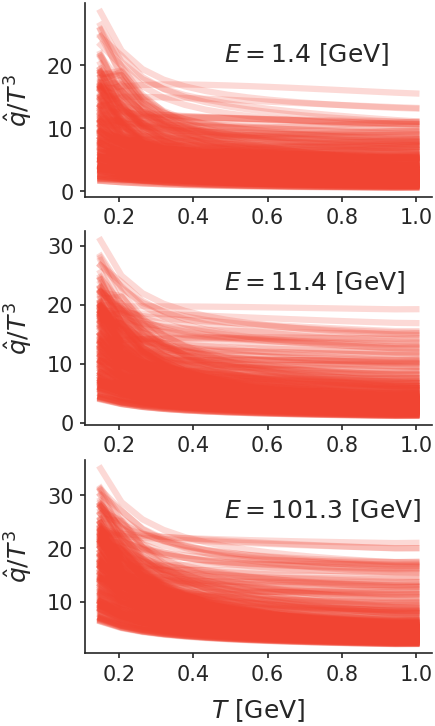
\includegraphics[width=.5\textwidth]{qhat_prior.png}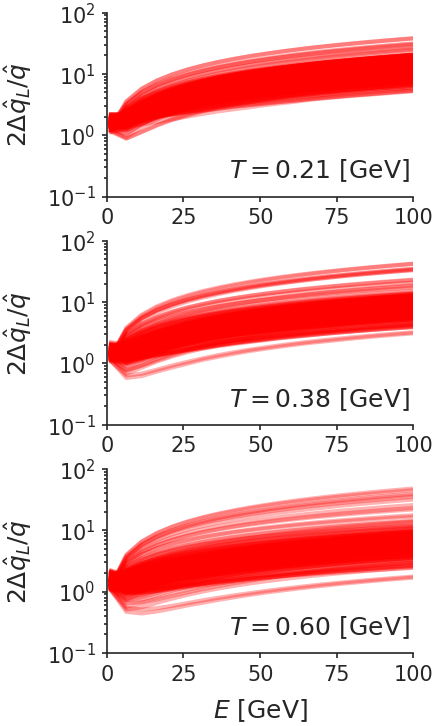
\includegraphics[width=.5\textwidth]{ER_prior.png}
\caption[Left: the prior range of the transport parameter $\hat{q}$ as funtion]{Left: the prior range of the transport parameter $\hat{q}$ as funtion of temperature at different heavy quark energy. Right: the prior range of the longitudinal diffusion parameter $\hat{q}_L$, plotted as ratio $2\hat{q}_L/\hat{q}$.}
\label{fig:new:design-qhat}
\end{figure}

\paragraph{Design and prior} 
We chosoe to give $\ln c, \ln R_v, \ln \mu, \ln a$ and $\ln b$ an uniform design and a uniform prior.
Therefore, the original parameter will have a non-uniform design and prior distribution.
The reason is that these parameters either cause a logarithmically slow change of the model prediction or their prior uncertainty is large that they are allowed to vary by orders of magnitude.
For example, the $\mu$ parameter enters the logarithmic running of $\alpha_s$ and we can rewrite the maximum possible $\alpha_s$ as,
\begin{eqnarray}
\alpha_{s,\max}(T) = \frac{2\pi}{9}\frac{1}{\ln(\mu) + \ln(\pi T/\Lambda_{\textrm{QCD}})}
\end{eqnarray}
Therefore, we assign a uniform prior to $\ln(\mu)$ so that $\alpha_s$ also varies notable within the prior range.
For the $c$ and $R_v$ parameter, we have seen in the previous benchmark calculation that the $R_{AA}$ and $v_2$ predictions depend fairly weakly on the choice of these parameters, therefore they are also given a logarithm prior.
For the $a$ and $b$ parameters, one notices that asymptotic largeness or smallness of these numbers do not change the value of $\Delta \hat{q}$ notably.
By applying the logarithmic prior, we can explore both the large and small limits of these numbers while still having enough design points to control the interpolation uncertainty in the physically interesting regions ($a$ and $b$ are of order one). 

We sample 250 design points and 50 validation points. 
Combining $\mu, K, p, q, a, b$ and $\gamma$, the prior region of the heavy quark transport parameters are plotted as a function of temperature and energy in figure \ref{fig:new:design-qhat}. 
On the left, the 250 design $\hat{q}$'s as function of temperatures are shown  (using charm mass for demonstration).
Each subplot shows a quark energy at $1.4$ GeV, $11.4$ GeV and $101.3$ GeV.
The prior range of $\hat{q}$ varies over an order of magnitude.
On the right of the figure, we show the ratio $2\hat{q}_L/\hat{q}$ to indicate the degree of anisotropy of the transport parameters.

The computations of the model on both the design points and the validation points are performed on the NERSC super-computing platform using over two million CPU hours.
The observables calculated on the prior are shown in figure \ref{fig:new:obs_prior_LHC} at LHC energy $\sqrt{s}$ = 5.02 TeV and in figure \ref{fig:new:obs_prior_RHIC} at RHIC energy $\sqrt{s} = 200$ GeV.
In addition to the LHC dataset used in the last calibration, we also include a dataset at RHIC energy measured by the STAR Collaboration \cite{Adamczyk:2017xur,Adam:2018inb}.
We choose two observables at RHIC, namely D meson $R_{CP}$ and $v_2$. 
The new one, $R_{CP}$, is defined as the $N_{\textrm{bin}}$ normalized ratio between the D meson yield in a smaller centrality class $C$ to a larger centrality class $P$,
\begin{eqnarray}
R_{\textrm{CP}} = \frac{dN_\textrm{C}/dp_T N_{\textrm{bin,P}}}{dN_\textrm{P}/dp_T N_{\textrm{bin,C}}}.
\end{eqnarray}
Using the nuclear data as a reference has the advantage of canceling certain theoretical uncertainties, such as the nuclear PDF (if its impact-parameter dependence is neglected) and possible modifications to the initial production mechanism in the nuclear environment.
A problem we found at RHIC energy is that even exploring a broad parameter range, the very low-$p_T$ $R_{CP}$ is not well covered by the calculation. 
This indicates the model will have to be improved in this region of $p_T$, possibly by a more up-to-date dynamical hadronization model.
Our temporary solution is to only include the STAR $R_{CP}$ data above $5$ GeV in the calibration.

\begin{figure}
\singlespacing
\centering
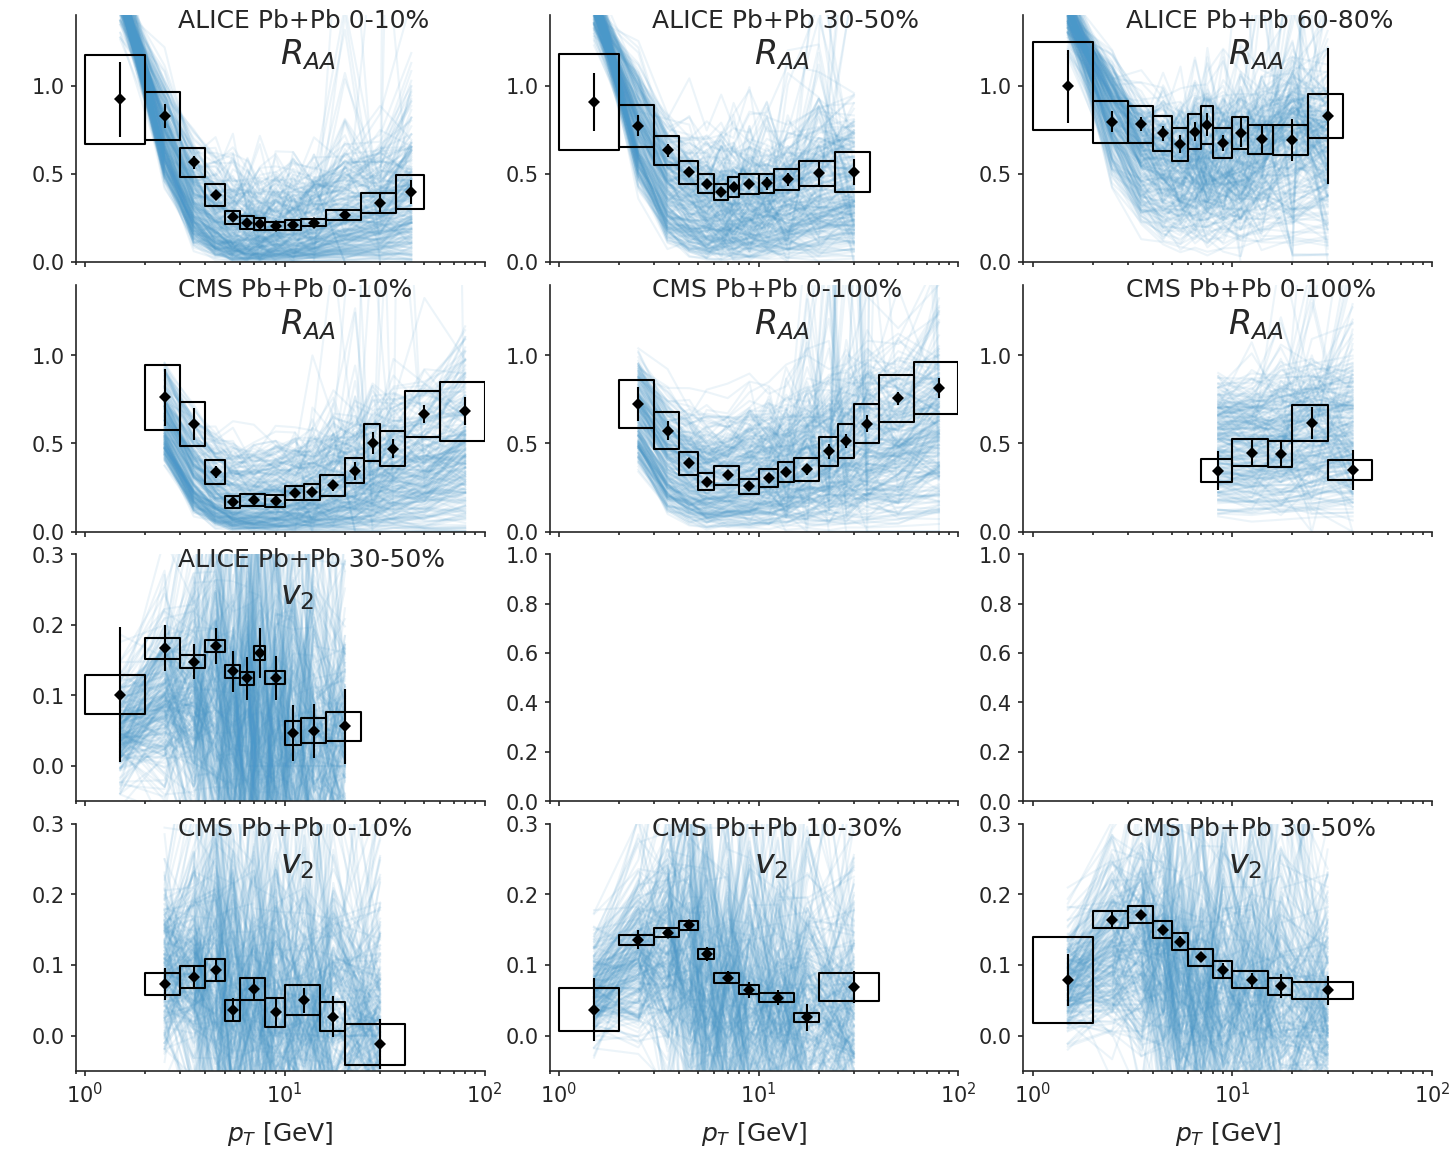
\includegraphics[width=\textwidth]{obs_prior_LHC.png}
\caption[The prior distribution of the calculated observables at LHC]{The prior distribution of the calculated observables at LHC energy compared to data.}
\label{fig:new:obs_prior_LHC}
\end{figure}

\begin{figure}
\singlespacing
\centering
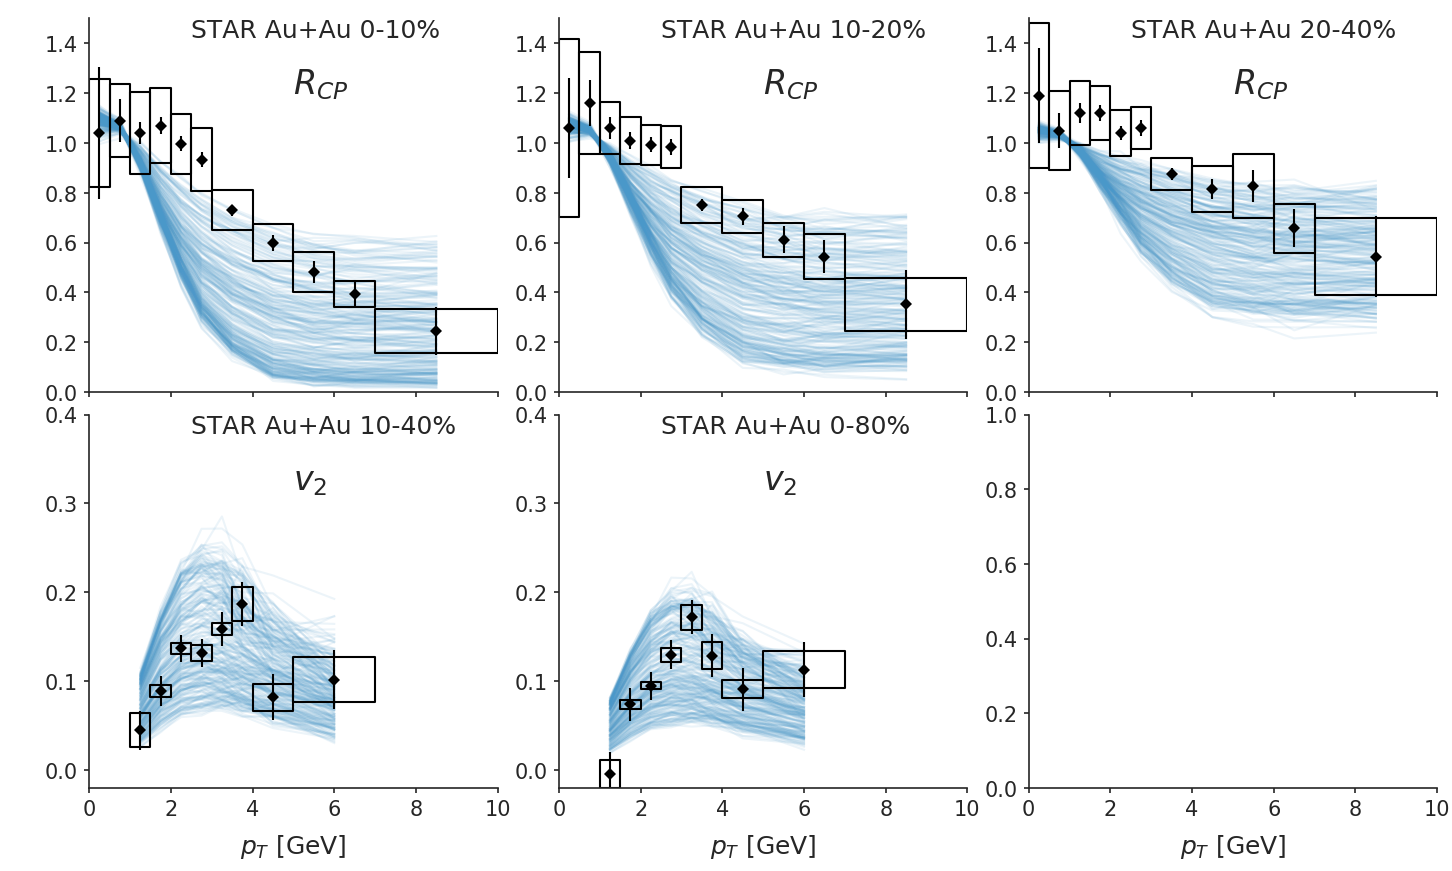
\includegraphics[width=\textwidth]{obs_prior_RHIC.png}
\caption[The prior distribution of the calculated observables at RHIC]{The prior distribution of the calculated observables at RHIC energy compared to data.}
\label{fig:new:obs_prior_RHIC}
\end{figure}

\paragraph{Emulator validation} 
The validation is performed by comparing the emulator trained on the 250 design points to the actual calculation on the 50 validation points.
We visualize the validation in figure \ref{fig:new:validation}.
In the top row, the emulated $v_2$ (left) and emulated $R_{AA}$ (right) are compared with the model calculations, and the data from different experiments and centrality has been labeled by different colors.
The emulated values strongly correlates with the true calculations around the the $y=x$ line.
Most points slightly miss the line, meaning the emulator is not 100\% accurate.
To see if the uncertainty is accounted for, we scatter plot the emulator's prediction uncertainty ($1\sigma$, $y$ axis) versus the absolute deviation between the prediction and the calculation (the $x$ axis).
The dashed line defines the shaded region where the true deviation is large than $\pm 3\sigma$.
We found that over $99\%$ of the prediction are within the $3\sigma$ region.
Therefore, for most cases the emulator correctly estimates its uncertainty  and therefore prevents over-fitting.

\begin{figure}
\singlespacing
\centering
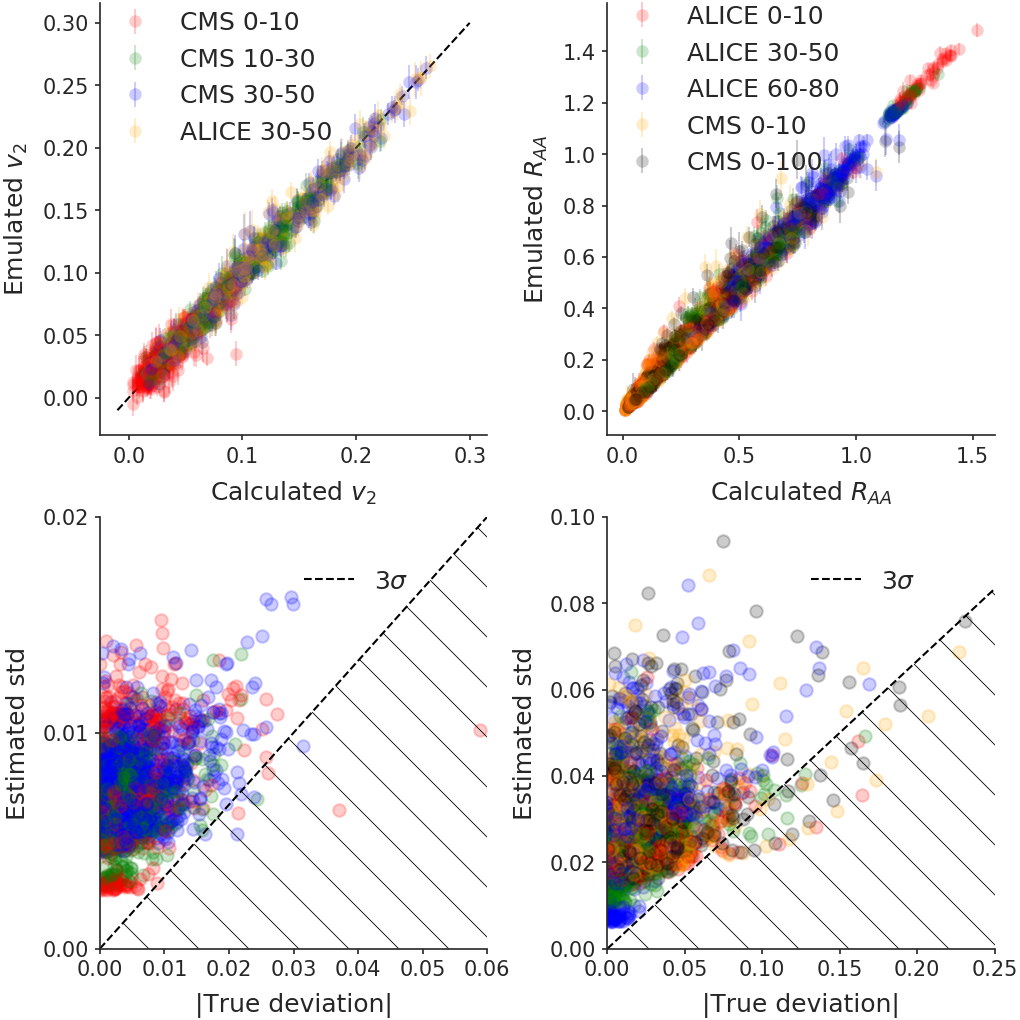
\includegraphics[width=.8\textwidth]{validation.png}
\caption[Validation of the emulators performance. The top two plots shows]{Validation of the emulators performance. The top two plots shows the correlation between the calculated quantities ($x$ variable) versus the emulated quantities ($y$ variable). The bottom two plots compare the GP's estimated standard deviation $\sigma$ of the prediction to the true deviation from the actual calculation. The dashed regions indicates where the true deviations have a larger than $3\sigma$ difference from the emulator's prediction.}
\label{fig:new:validation}
\end{figure}

\paragraph{Covariance matrix} 
From chapter \ref{chapter:bayes}, the covariance matrix has the structure
\begin{eqnarray}
\Sigma = \Sigma_{\textrm{emulator}} + \Sigma_{\textrm{truncation}} + \Sigma_{\textrm{stat}} + \Sigma_{\textrm{sys}} + \Sigma_{\textrm{model, sys}} 
\end{eqnarray}
The construction of these terms is straight forward, except for the systematic covariance $\Sigma_{\textrm{sys}}$ of the experimental data.
Usually, experiments publish the marginalized uncertainty on each observable point $\delta y_{sys}$ (for example, $R_{AA}$ of a certain centrality at a single $p_T$ bin), and may specify the nature of the uncertainty as ``correlated'' or ``uncorrelated''.
The correlation among uncertainties is important as it directly affects the interpretation of the quality of fit.
For instance: a fit with $+5\%$ deviations on each of the $N$ data points will be penalized by a factor $e^{-N(0.05 y)^2/\delta y^2}$, assuming uncorrelated uncertainty; while it will only be penalized by $e^{-(0.05 y)^2/\delta y^2}$ if one assumes fully correlated uncertainty.
This is because fully correlated uncertainty allows data to systematically deviate from a trend.

However, we the lack the information to construct the full covariance matrix from $\delta y_{sys}$.
In this study, we simply parametrize the correlation as function of observables (labeled by $\alpha, \beta \in \{R_{AA}, v_2, R_{CP}\}$), centrality labeled by $m,n$ and transverse momentum (labeled by $i,j$),
\begin{eqnarray}
\mathbf{\Sigma}_{\textrm{sys}} = \delta_{\alpha\beta} C_{mn}  \exp\left\{-\frac{1}{2 L_{\textrm{corr}}^2} \left(\ln\frac{p_{T, i}}{p_{T, j}}\right)^2 \right\} \times \sigma^{\alpha m}_{\textrm{sys}, i}\sigma^{\beta n}_{\textrm{sys}, j}.
\end{eqnarray}
So, the covariance is zero if there are different observables or measurements from different experiments or different particle species.
The centrality correlation $C_{mn}$ is only applied to $R_{AA}$ and $R_{CP}$ as these quantities shares the same baseline reference across different centrality, so a fraction of their uncertainty must be correlated across-centrality. 
By default, $C_{m=n}=1$ and $C_{m\neq n}=0.3$.
The correlation in the $p_T$ dimension is assumed to be a Gaussian in the $\ln p_T$ space with correlation length $L_{\textrm{corr}}$.
We use $\ln p_T$ based on the consideration that the original uncertainty should not be sensitive to the linear change of $p_T$ as the there is no other scale present.
The default correlation length is $1$, meaning the uncertainty is effectively uncorrelated with measurements at a $p_T$ $2.7$ times larger or smaller.
Finally, this correlation modulation is applied to the completely correlation case of the systematic uncertainty $\sigma^{\alpha m}_{\textrm{sys}, i}\sigma^{\beta n}_{\textrm{sys}, j}$.
This construction is entirely parametric, except for the direct experimental inputs $\sigma^{\alpha m}_{\textrm{sys}, i}$.
We hope that future measurements will provide more information on the co-variance structure of the published systematic uncertainties.

What we have done is to parametrize the unknown experimental covariance matrix by a reasonable ansatz using two parameters $C$ and $L_{\textrm{corr}}$.
One may try selecting different values $C$ and $L_{\textrm{corr}}$ to do a Bayesian analysis to investigate whether the calibrated parameters are sensitive to these choices.
However, since neither of these values is superior than the rest due to the lack of knowledge, the uncertainty from different choices should be considered as another uncertainty to the model-to-data comparison.
In the Language of the Bayesian analysis, we treat $L_{\textrm{corr}}$ (the $C$ parameter is fixed to the default values for simplicity) as a hyperparameter that appears in the definition of the likelihood function, and use the MCMC to marginalize this parameter when focusing on other parameters.
It is given a uniform prior probability distribution within $0.2 < L_{\textrm{corr}} < 2.0$.
This range corresponds to $1\sigma$ reduction of the correlation once $p_T$ is multiplied a factor of $1.2$--$7.4$.
Meanwhile, the posterior distribution also infers the probability distribution of $L_{\textrm{corr}}$.
We can compare this inference to future experimental estimations of the uncertainty correlation for a consistency check.

\begin{figure}
\singlespacing
\centering
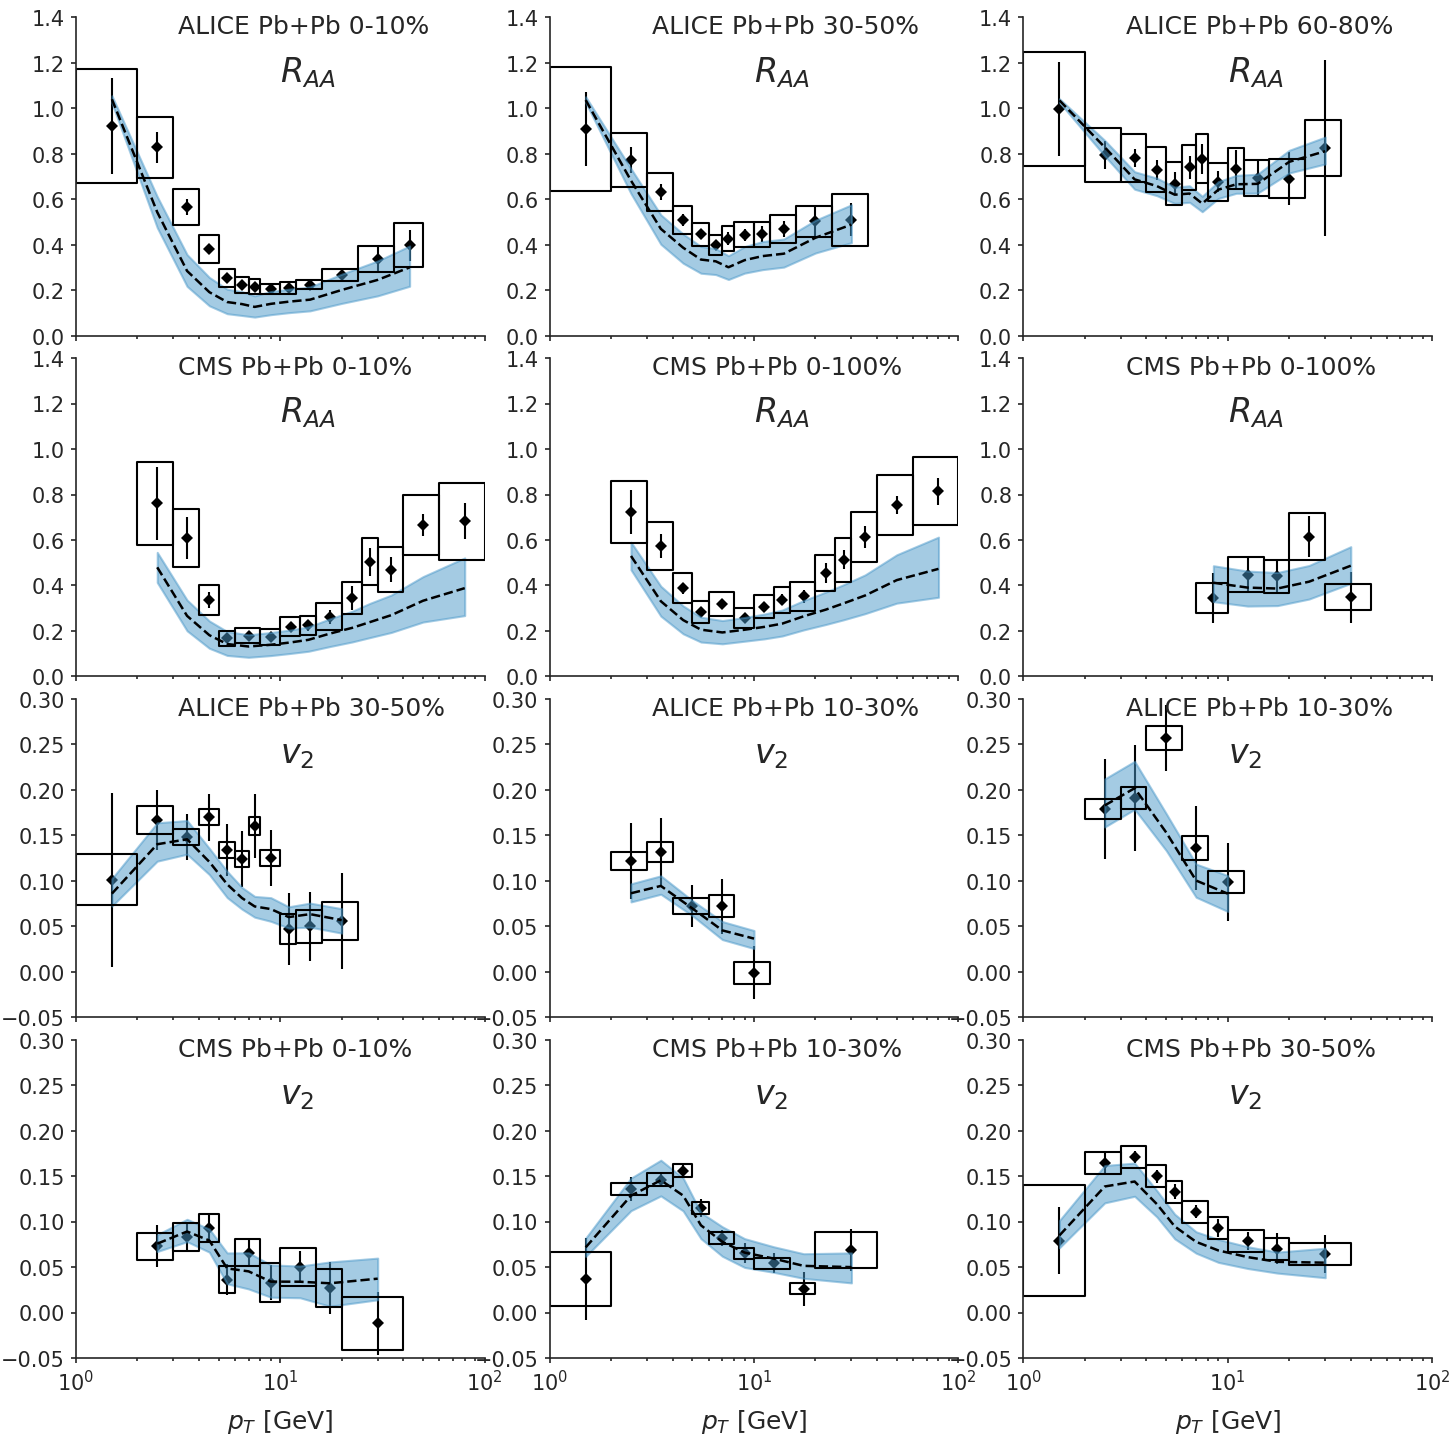
\includegraphics[width=\textwidth]{obs_posterior_LHC.png}
\caption[The 90\% credible region (blue bands) of the posterior distribution]{The 90\% credible region (blue bands) of the posterior distribution of the observables at the LHC energy. Black dashed lines are the median prediction.}
\label{fig:new:obs_posterior_LHC}
\end{figure}

\paragraph{Posterior observables} The global level of agreement between the calibrated model and the data is shown in figure \ref{fig:new:obs_posterior_LHC} at the LHC energy, and figure \ref{fig:new:obs_posterior_RHIC} at the RHIC energy.
The black dashed lines show the median prediction, while the blue bands stands for $90\%$ credible region.
We remind the reader that because the model predicts anti-correlation between $R_{AA}$ and $v_2$, the lower and upper bounds of the uncertainty bands are also anti-correlated.
For example, a line that is close to the higher bounds in $R_{AA}$ is likely to be lose to the lower bounds in $v_2$.

The shape of the $D$-meson and the $B$-meson $R_{AA}$ and $D$-meson $v_2$ at the LHC energy are described by the calibrated model, while the absolute values of $R_{AA}$ are systematically below the data, so the $R_{AA}$-$v_2$ is not entirely solved in the current level of modeling.
A large separation between the event-engineered $v_2$ is observed and is in a good agreement with data.
This means our model correctly accounts for the heavy-flavor response on the event-by-event geometry fluctuation of the medium.
At RHIC energy, $v_2$ is well described.  
The magnitude of $R_{CP}$ at $p_T> 5$ GeV \footnote{\singlespacing  Remember that the model is calibrated on the three data points above $p_T=5$ GeV} and its centrality dependences are correctly reflected, though the $p_T$-shape is too flat compared to the data.

\begin{figure}
\singlespacing
\centering
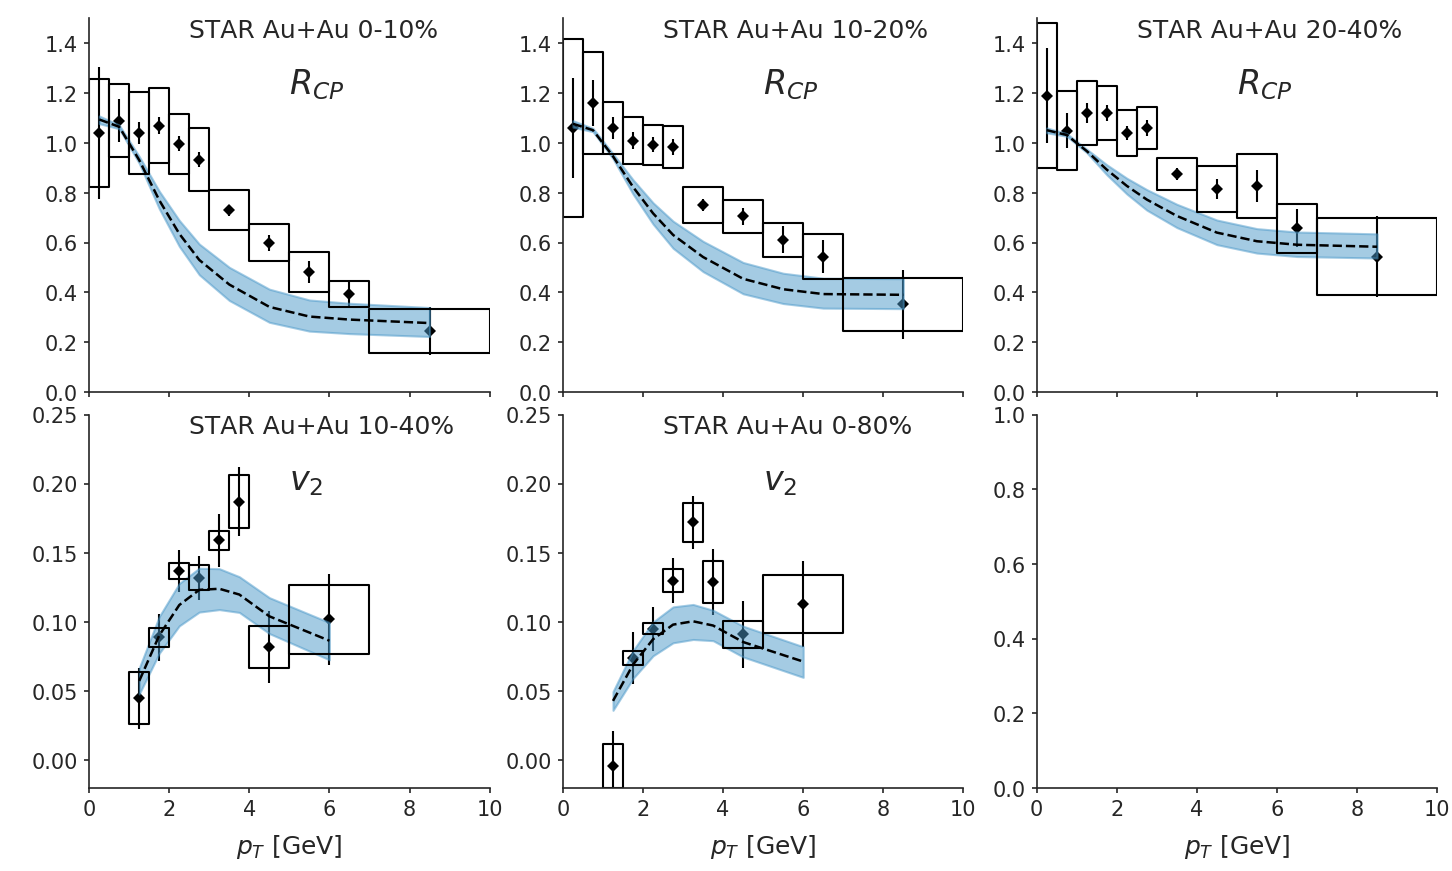
\includegraphics[width=\textwidth]{obs_posterior_RHIC.png}
\caption[The 90\% credible region (blue bands) of the posterior distribution]{The 90\% credible region (blue bands) of the posterior distribution of the observables at the RHIC energy. Black dashed lines are the median prediction.}
\label{fig:new:obs_posterior_RHIC}
\end{figure}

\begin{figure*}
\centering
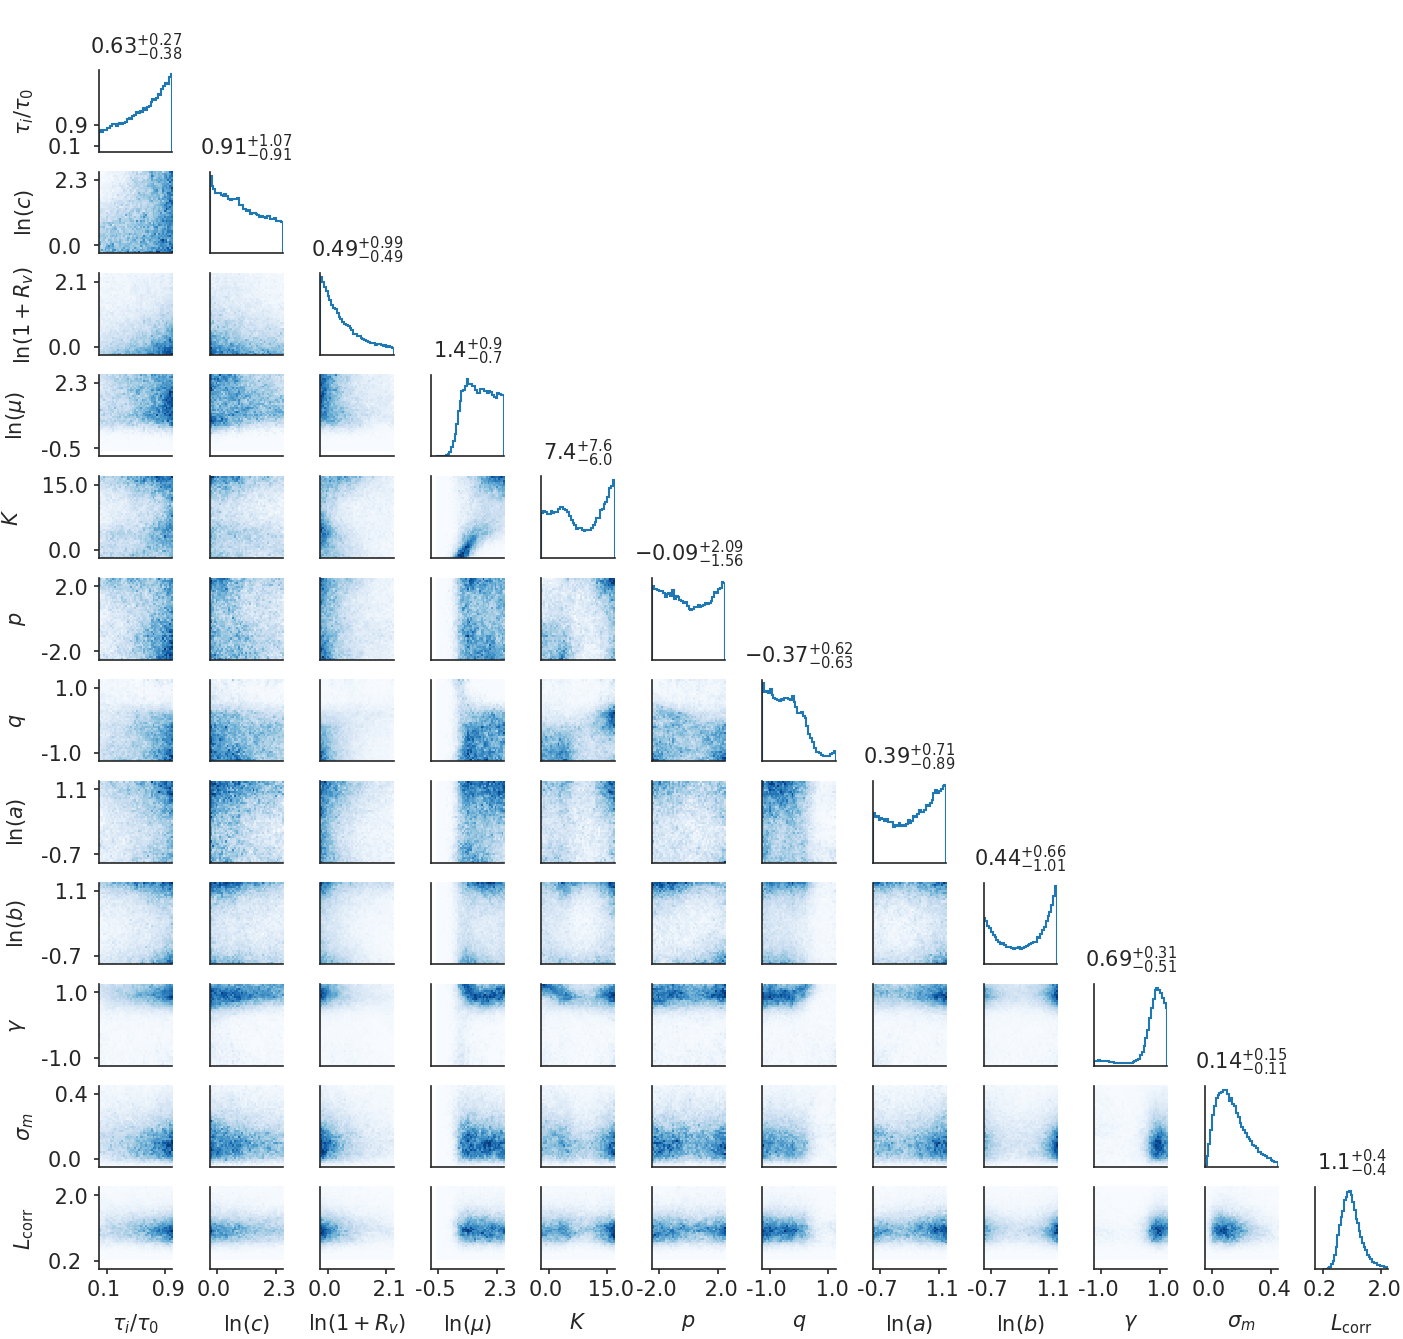
\includegraphics[width=\textwidth]{new-posterior.png}
\caption[The single-parameter posterior distributions (diagonal plots) and]{The single-parameter posterior distributions (diagonal plots) and two-parameter joint posterior distributions (off-diagonal plots).}
\label{fig:new:posterior}
\end{figure*}

\paragraph{Posterior distribution of parameters} Figure \ref{fig:new:posterior} shows the single parameter posterior (diagonal plots) and two-parameter-joint posterior distributions (off-diagonal plots) of the 10 model parameters, plus the model systematic uncertainty parameter ($\sigma_m$).
Both the $\ln\mu$ parameter which controls the perturbative coupling and the $K$ parameter which controls the magnitude of parametric diffusion have rather broad distributions.
But looking at the correlation between these two parameters, we find that the high-likelihood parameter values can either be around $\mu\sim 1.5, K\sim 0$ or around $\mu\sim 8, K\sim 15$.
So that a similar level agreement with data can either be achieved with a more perturbative-driven physics or a more parametric modeling using diffusion.
Note that since the origin of this parametric diffusion can also be coming a high-order correction to $\hat{q}$ from a weakly-coupled theory, we cannot immediately interpret a large $K$ value as a large non-perturbative effect.

The resulting posterior of $\alpha_s$ is plotted in figure \ref{fig:new:posterior-alphas}, the median value of $\alpha_s$ at $Q=\mu\pi T$ varies from 0.3 to 0.22 for the relevant temperature range $0.15 < T < 0.5$ GeV, corresponding to $g\sim 2$.
Compared to the previous extraction, the preferred in-medium coupling strength is smaller and is closer to the phenomenological values used by other studies \cite{Burke:2013yra}.
However, the coupling is still large compared to the weakly coupled assumption $g\ll 1$.
This $\alpha_s$ does not stand for the strength of all the probe-medium interaction, recalling that there is a significant parametric diffusion contribution to the elastic energy loss.
For radiative processes, though the $1\rightarrow 2$ splitting vertex explicitly uses this $\alpha_s$, the strength of the LPM effect is again controlled by the elastic broadening.

\begin{figure}
\singlespacing
\centering
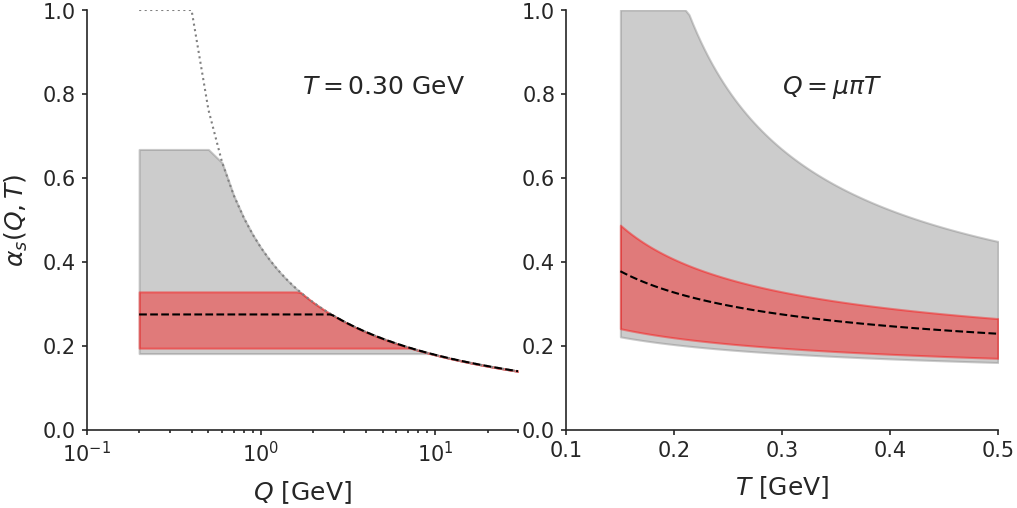
\includegraphics[width=.8\textwidth]{alpha_s_posterior.png}
\caption[Left plot: the scale dependence of the running coupling constant at]{Left plot: the scale dependence of the running coupling constant at $T=0.3$ GeV. Right plot: the temperature dependence of running coupling evaluated at the cut-off scale $Q=\mu\pi T$. The red bands are generated using 90\% credible region of the $\mu$ parameter; the gray bands are the prior distributions; and the black dashed lines are median predictions.}
\label{fig:new:posterior-alphas}
\end{figure}

The calibration suggests a late energy loss starting time with a medium value around 0.6 of the $\tau_{\textrm{hydro}}$.
The switching scale parameter does not have a strong preference as long as it is not too large, which is consistent with our model construction that physical processes should only weakly depend on this switching scale between diffusion and scattering modeling.
The posterior matching parameter $R_v$ tends a small value, with a median value $0.6$, meaning a matching between vacuum-like and medium-induced showers around $\Delta k_\perp^2 \sim 0.6 Q^2$.

\begin{figure}
\singlespacing
\centering
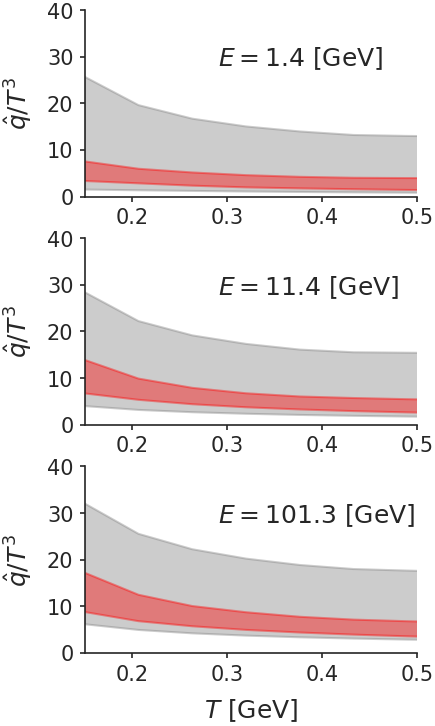
\includegraphics[width=.5\textwidth]{qhat_posterior.png}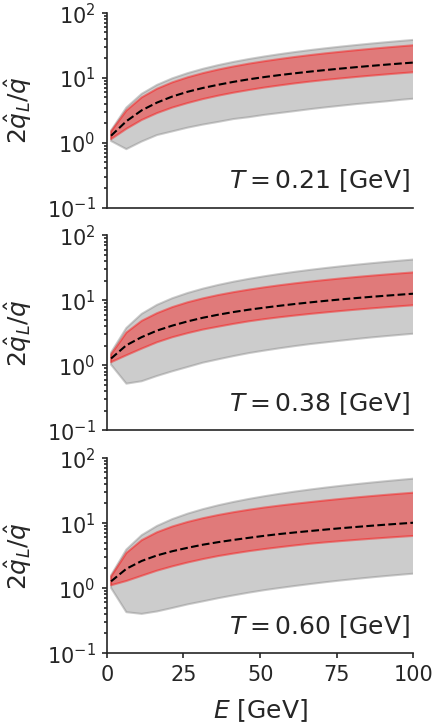
\includegraphics[width=.5\textwidth]{ER_posterior.png}
\caption[The 90\% credible region of the charm quark transport coefficients]{The 90\% credible region of the charm quark transport coefficients (left plot) and of the longitudinal transport parameter (right plot) are shown in red. The prior range are shown in gray. The results are also compared to the previous JET Collaboration extraction of the light quark transport parameters at $p=10$ GeV (black symbols). }
\label{fig:new:posterior-qhat}
\end{figure}

The posteriors of $p, q, a, b, \gamma$ cannot be easily explained individually. 
It is more instructive to directly look at the posteriors of the transport coefficients $\hat{q}, \hat{q}_L$.
We plot the 90\% credible range (red bands) of charm quark $\hat{q}, \hat{q}_L$ on top of their prior range (gray band) in figure \ref{fig:new:posterior-qhat}.
The values of $\hat{q}$ at $E=10.4$ GeV are found to be comparable to earlier extractions of the light quark $\hat{q}$ by the JET Collaboration \cite{Burke:2013yra} \footnote{\singlespacing  Note that the JET Collaboration extracts the light quark $\hat{q}$. However, at $p_T = 10$ GeV, the mass effect of the charm is small and these two numbers should be comparable.}.
We also present a first extraction of the longitudinal transport parameter $\hat{q}_L$. 
The longitudinal transport is quite anisotropic when compared to $\hat{q}$.

For the heavy quark spatial diffusion constant, since it is related to $\hat{q}$ in the zero momentum limit, our extraction is essentially an extrapolation of the parametrization and can be sensitive to the detailed choice of the ansatz.
Nevertheless, the extraction (red band for 90\% credible region) is compared to various lattice calculations \cite{Banerjee:2011ra,Ding:2012sp,Francis:2015daa} in  figure \ref{fig:new:posterior-Ds}.
Our extraction for both the charm and bottom quark spatial diffusion constants is similar, and is consistent with lattice calculations in the static / infinitely heavy limit of the heavy quark.
While the lattice calculation of dynamical charm quarks gives a much lower value of $D_s$.
One may expect that our phenomenological extraction should give a similar separation between bottom and charm flavor, as the bottom is more than three times heavier.
However, we found that the mass dependence in the elastic part of our model is relatively weak. 
First, the mass only affects the phase-space integration of $t$-channel exchange perturbative scattering.
Second, we are using the heavy-quark limit that it does not depend on mass for the diffusion parameter of the weakly coupled theory, 
Finally, mass only enters the parametric diffusion part through a combination $E/T$, which is approximately $M/T$ at low momentum, since both charm and bottom mass are already much higher than the typical temperature, therefore the parametric part also introduces only a weak flavor dependence.
In the future, one may seek a more physically motivated flavor dependence parametrization of the transport parameters.

\begin{figure}
\singlespacing
\centering
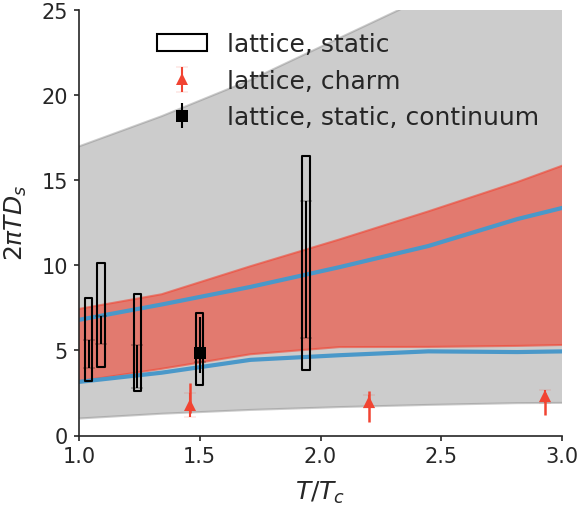
\includegraphics[width=.7\textwidth]{Ds_posterior.png}
\caption[The 90\% credible region of the spatial diffusion constant defined]{The 90\% credible region of the spatial diffusion constant defined in the zero momentum limit. Prior range is indicated by the gray band. The posterior of charm and bottom flavor are shown as red band and blue boundary receptively. It is compared to lattice QCD evaluation in references \cite{Banerjee:2011ra} (black boxes), \cite{Francis:2015daa} (the black dot) and \cite{Ding:2012sp} (red triangles).}
\label{fig:new:posterior-Ds}
\end{figure}